\documentclass[a4paper, 10pt]{article}
\usepackage[utf8]{inputenc} % Change according your file encoding
\usepackage{graphicx}
\usepackage{url}
\usepackage{listings}
\usepackage{xcolor}
\usepackage{caption}
\usepackage{multirow}
\usepackage{pgfplots}
\usepackage{float}
\usepackage[parfill]{parskip}
\restylefloat{table}
\graphicspath{ {./images/} }


%opening
\title{Seminar Report: OPTY}
\author{\textbf{Juan Pablo Royo Sales, Alicia Vila Rodriguez and} \\\and \textbf{Sergi Palomas Martinez}}
\date{\normalsize\today{}}

\begin{document}

\maketitle

\section{Introduction}

In the context of distributed systems, it is assumed that multiple transactions can happen in the same time and on the same file. Therefore, methods for solving conflicting transactions are numerous and have been improved since the beginning. In this report, we have emulated a system where multiple clients are accessing (R/W) to a set of files (entries). We will use the \textit{Optimistic concurrency control} algorithm with backward validation. Different number of operations, clients, entries and different read/write ratios will be tested to show how this parameters can affect the performance of the algorithm.

\section{Code Organization}


\subsection{Optimistic concurrency control experiments}

All the source code can be found in the cpds-opty/src/ folder.\\\\
For the experiments using the \textit{Optimistic concurrency control}, you can find a new module called \textit{experiments.erl} where we have defined different functions for making the experiments execution easier.

\subsection{Timestamp ordering experiments}

Regarding the analysis of other concurrency control techniques (section 5 of the statement), we have used the \textit{Timestamp ordering} algorithm code provided by the wiki. We have added a new module called \textit{experiments\_timey.erl} to execute the same experiments as in the section 3 of the statement. \\\\
All the source code can be found in the cpds-opty/Timey/src/ folder.

\section{Performance}

\subsection{Experiments and analysis}

\subsubsection{\textit{i)} What is the impact of each of these parameters on the
success rate?}

\begin{enumerate} 
\item \textbf{Question:} Different number of concurrent clients\\\\
    
\begin{minipage}[hbt!]{\linewidth}
  \centering
  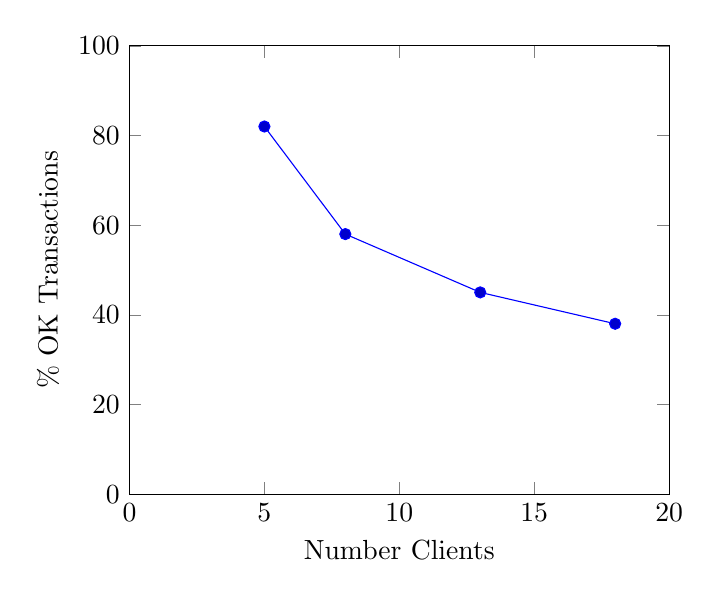
\begin{tikzpicture}
    \begin{axis}
      [
      xlabel={Number Clients},
      ylabel={\% OK Transactions},
      xmin=0, xmax=20,
      ymin=0, ymax=100,
      scaled x ticks = true,
      scaled y ticks = true,
      legend style={nodes=right},
      ]
      \addplot coordinates {
        (5, 82)
        (8, 58)
        (13, 45)
        (18, 38)
      };
    \end{axis}
  \end{tikzpicture}
  \captionof{figure}{Relation between number of clients and OK Transactions}
  \label{fig:rel_cli_tx}
\end{minipage}

\textbf{Answer:} As shown in the plot \ref{fig:rel_cli_tx}, the increase on the number of concurrent clients running in the systems makes the success rate drop. Which is what we expected since the number of operations is also increasing. Thus, the probability of conflicting transactions is higher.

\item \textbf{Question:} Different number of entries in the store\\\\
  \begin{minipage}[hbt!]{\linewidth}
    \centering
    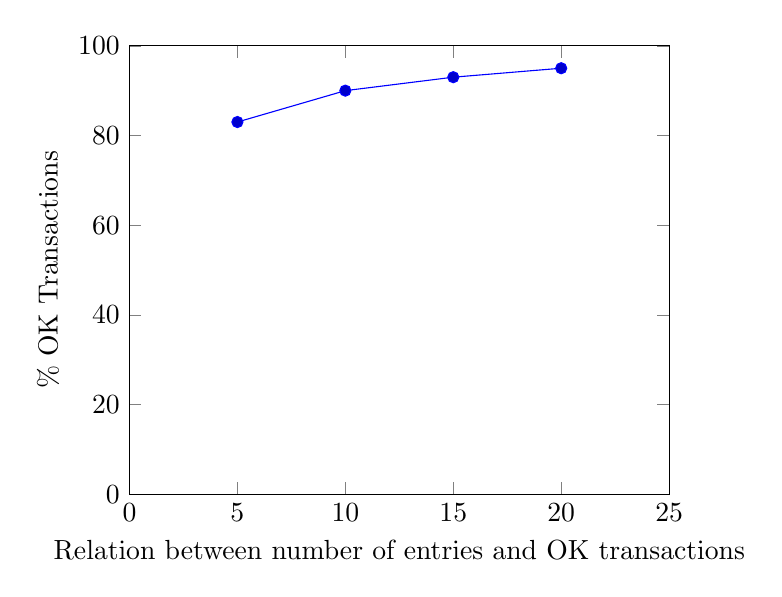
\begin{tikzpicture}
      \begin{axis}
        [
        xlabel={Relation between number of entries and OK transactions},
        ylabel={\% OK Transactions},
        xmin=0, xmax=25,
        ymin=0, ymax=100,
        scaled x ticks = true,
        scaled y ticks = true,
        legend style={nodes=right},
        ]
        \addplot coordinates {
          (5, 83)
          (10, 90)
          (15, 93)
          (20, 95)
        };
      \end{axis}
    \end{tikzpicture}
    \captionof{figure}{Relation between number of entries and OK transactions}
    \label{fig:rel_entries_tx}
  \end{minipage}

\textbf{Answer:} The plot \ref{fig:rel_entries_tx} shows how the percentage of OK transactions increase as we add more entries. The probability of two (or more) clients to be accessing on the same entry is less, therefore, reducing the conflicting transactions.

\item \textbf{Question:} Different number of Read and Writes Operations per Transaction\\\\

  \begin{minipage}[hbt!]{\linewidth}
    \centering
    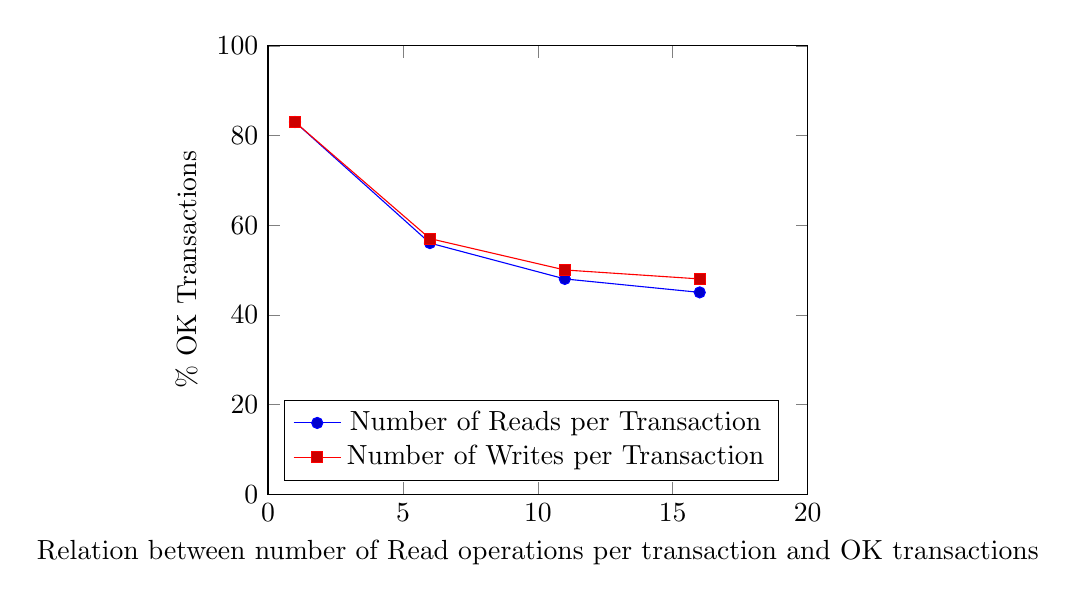
\begin{tikzpicture}
      \begin{axis}
        [
        xlabel={Relation between number of Read operations per transaction and OK transactions},
        ylabel={\% OK Transactions},
        xmin=0, xmax=20,
        ymin=0, ymax=100,
        scaled x ticks = true,
        scaled y ticks = true,
        legend pos= south west,
        ]
        \addplot coordinates {
          (1, 83)
          (6, 56)
          (11, 48)
          (16, 45)
        };
        \addplot coordinates {
          (1, 83)
          (6, 57)
          (11, 50)
          (16, 48)
        };
        \addlegendentry{Number of Reads per Transaction}
        \addlegendentry{Number of Writes per Transaction}
      \end{axis}
    \end{tikzpicture}
    \captionof{figure}{Relation between number of Read operations per transaction and OK Transactions}
    \label{fig:rel_read_and_writes_tx}
  \end{minipage}


\textbf{Answer:} In plot \ref{fig:rel_read_and_writes_tx},  we can see how the percentage of success decrease as number of Read operations per transaction is bigger. Obviously, more Read operations increase the probability of conflicts in each successive operation. The same goes when we increase the number of Write operations (plot TODO) since the following Read conflict probability is increased. Thus, reducing the OK transactions percentage.

\item \textbf{Question:} Different Ratio of Read/Write Operations for a fixed
  amount of operations per transaction \\\\

 \begin{minipage}[hbt!]{\linewidth}
    \centering
    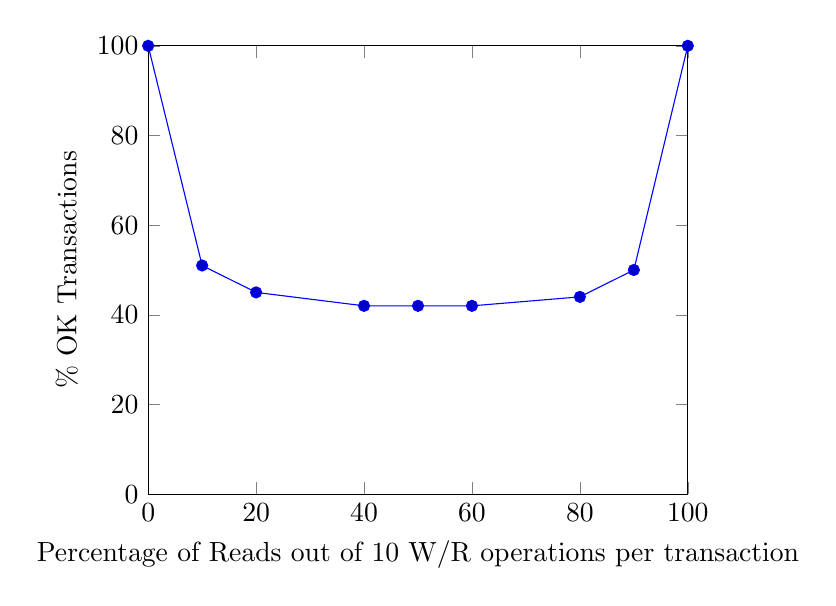
\begin{tikzpicture}
      \begin{axis}
        [
        xlabel={Percentage of Reads out of 10 W/R operations per transaction},
        ylabel={\% OK Transactions},
        xmin=0, xmax=100,
        ymin=0, ymax=100,
        scaled x ticks = true,
        scaled y ticks = true,
        legend style={nodes=right},
        ]
        \addplot coordinates {
          (0, 100)
          (10, 51)
          (20, 45)
          (40, 42)
          (50, 42)
          (60, 42)
          (80, 44)
          (90, 50)
          (100, 100)
        };
      \end{axis}
    \end{tikzpicture}
    \captionof{figure}{Relation between ratio of Read/Write operations per transaction and OK transactions}
    \label{fig:rel_read_writes_tx}
  \end{minipage}


\textbf{Answer:} In plot \ref{fig:rel_read_writes_tx}, it is shown how the ratio of Read and  Write operations affect at our system. Discarding the extreme values ( all Reads or all Writes) we see some stable and mirror results. The number of Read operations increase the probability of conflict but the increase of Write operations increase the Probability of a conflict on the following Read (which, again, increase the probability of conflict.

  
\item \textbf{Question:} Different percentage of accessed entries with respect
  to the total number of entries

  \begin{minipage}[hbt!]{\linewidth}
    \centering
    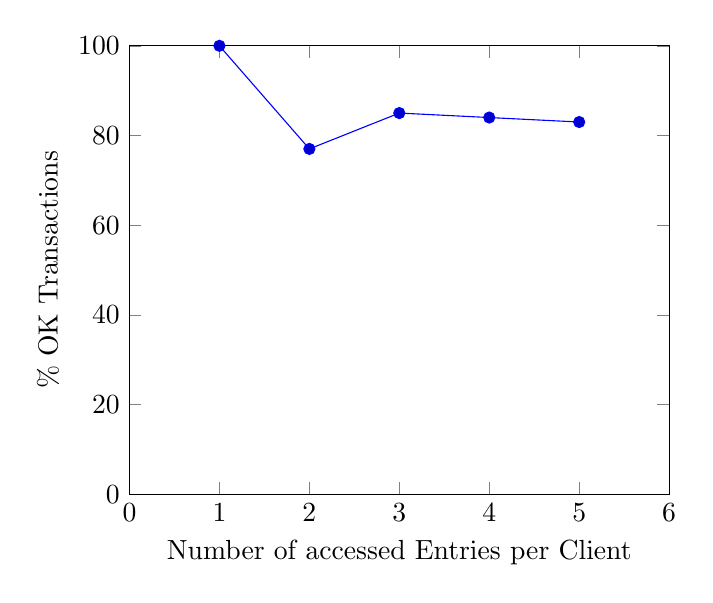
\begin{tikzpicture}
      \begin{axis}
        [
        xlabel={Number of accessed Entries per Client},
        ylabel={\% OK Transactions},
        xmin=0, xmax=6,
        ymin=0, ymax=100,
        scaled x ticks = true,
        scaled y ticks = true,
        legend style={nodes=right},
        ]
        \addplot coordinates {
          (5, 83)
          (4, 84)
          (3, 85)
          (2, 77)
          (1, 100)
        };
      \end{axis}
    \end{tikzpicture}
    \captionof{figure}{Relation between number accessed Entries per Client and OK transactions}
    \label{fig:rel_accessed_entries_tx}
  \end{minipage}

  \textbf{Answer:} Plot \ref{fig:rel_accessed_entries_tx} shows the Relation
  between the performance of our system when the number of accessed entries per
  client is increased. It is shown that if each client has only access to one
  entry, the number conflictive operations is zero. But as we increase the
  size of the allowed subset of accessed entries per client, the number of
  shared entries between clients is also increased. Thus, the probability of conflicts is also bigger.
 
\end{enumerate}

\subsection{Is the number of success different on each Client}
Yes but only it is only notable when the number of accessed entries per client is changed. The accessed entries is initialized randomly for each client and some of them may have to share more/less entries. Therefore, this affects at the individual client success.

\section{Distributed Execution}

We have adapted Erlang code in order to run either remote or in local mode.
\\\\
Now \lstinline|opty:start(...)| function receives 1 parameter more at the
beginning which is the $Mode$ that can be $local \mid remote$. 
\\\\
In order to run it in \textbf{remote} mode we need to do the following steps:

\begin{itemize}
\item First Start \textbf{erlang} instance with remote mode for clients, which
  includes also Handlers of the clients.

\begin{lstlisting}
\$ erl -sname opty-client -noshell
\end{lstlisting}

\item After that we can run the program in remote mode

\begin{lstlisting}
\$ erl -sname opty-srv -remsh opty-client
Eshell V10.5.2  (abort with ^G)

(paxy-acc@My-Machine)1> opty:start(remote, 5,3,2,2,3,3).
\end{lstlisting}

\item In the following figure \ref{fig:remote} we can see this execution on remote mode. The
  screen was split into 2, to show in the above section it is the Erlang's client
  instance running, and bellow the Server.

  \begin{minipage}[t]{\linewidth}
    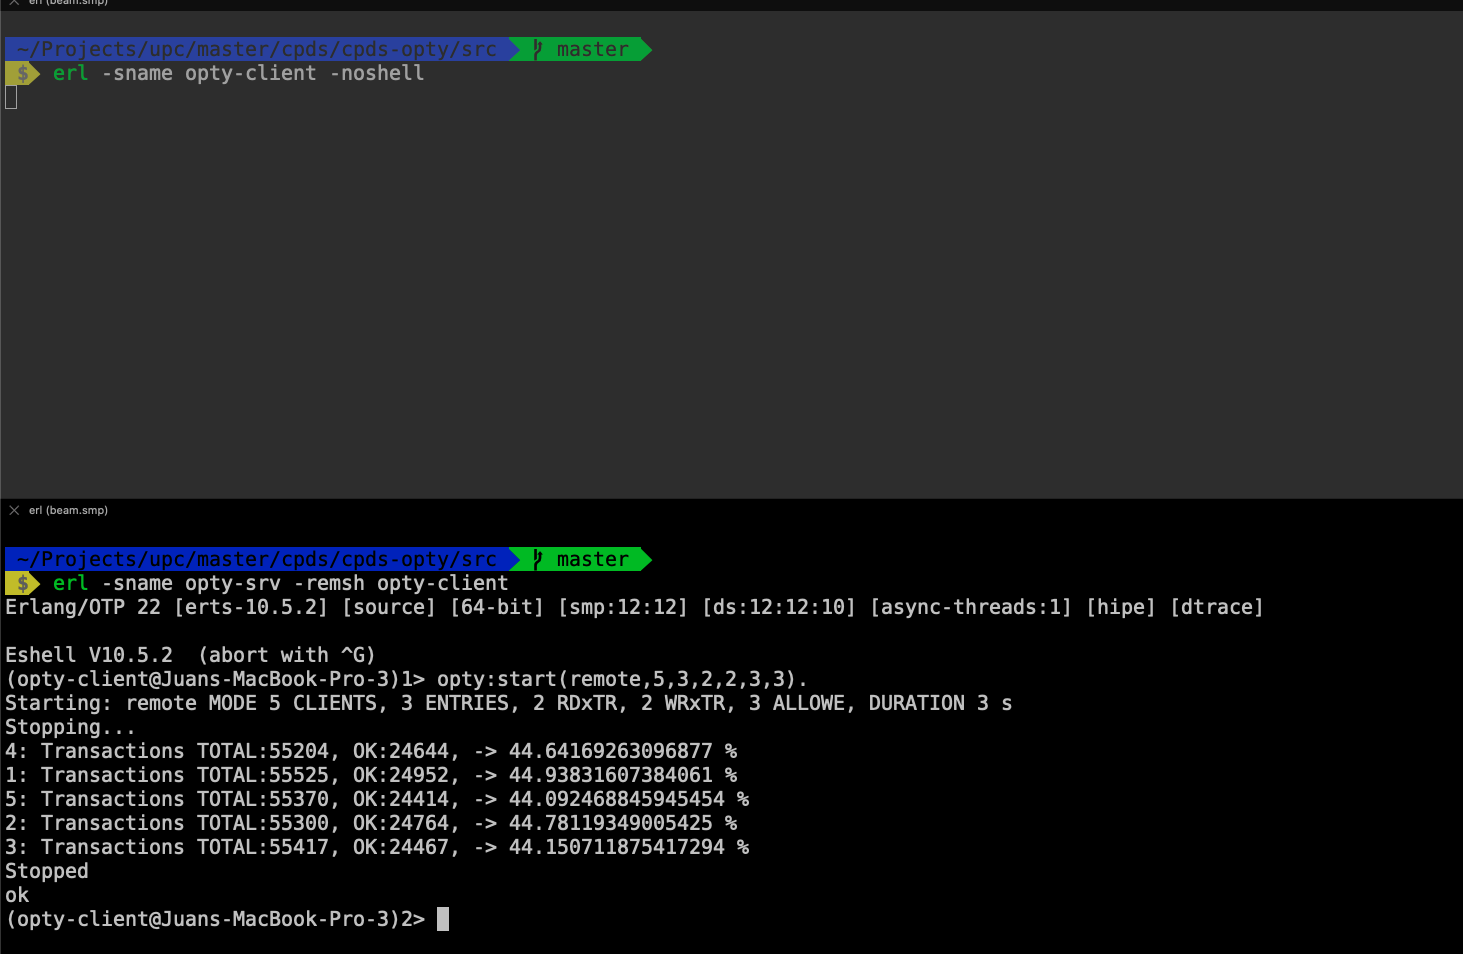
\includegraphics[width=\textwidth]{remote}
    \captionof{figure}{Remote execution of \lstinline|opty:start(remote,
      5,3,2,2,3,3)|}
    \label{fig:remote}
  \end{minipage}

\end{itemize}

\textbf{Open Question: } If we run this in a distributed Erlang network, where
  is the handler running?\\
\textbf{Answer: } The handler is running with the client Erlang instance because
it has an spawn-link with the clients.

\section{Timestamp ordering comparison}

Regarding the section 5 of the statement, we have chosen to do the comparison of the previous experiments with the \textit{Timestamp ordering} algorithm. The code we used is the one provided by the wiki. As the teacher said in the last class concerning this section, we have not modified the code, we have only performed different experiments to compare both algorithms. For this reason, we have only compared from the \textit{i)} to the \textit{v)} experiment.

\subsection{Experiments and analysis}

\begin{enumerate}
\item \textbf{Question:} Different number of total clients\\\\


\begin{minipage}[H]{\linewidth}
  \centering
  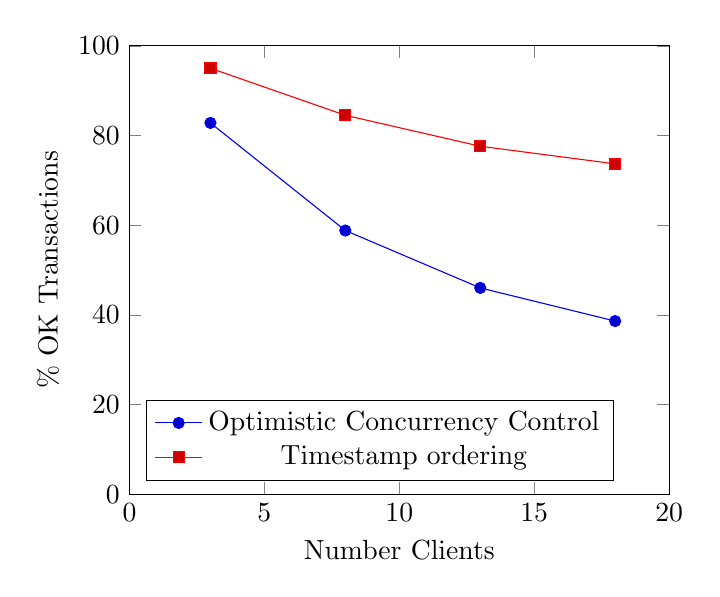
\begin{tikzpicture}
    \begin{axis}
      [
      xlabel={Number Clients},
      ylabel={\% OK Transactions},
      xmin=0, xmax=20,
      ymin=0, ymax=100,
      scaled x ticks = true,
      scaled y ticks = true,
      legend pos= south west,
      ]
      \addplot coordinates {
      (3,82.8)
      (8,58.8)
      (13,46)
      (18,38.6)
     };
     \addplot coordinates {
     (3,95)
     (8,84.5)
     (13,77.6)
     (18,73.67)
    };
    \addlegendentry{Optimistic Concurrency Control}
    \addlegendentry{Timestamp ordering}
    \end{axis}
  \end{tikzpicture}
  \captionof{figure}{Relation between number of clients and Ok Transactions}
  \label{fig:timey_graph_clients}
\end{minipage}

\textbf{Answer:} Is clear in the graphic that both algorithms decrease their
success rate when the number of clients get bigger. That is a logical behaviour,
so for attending more clients doing their transactions there are more concurrent
operations and that may cause more aborted transactions. Comparing both algorithms, clearly \textit{Timestamp ordering} get better success rate for all the different cases.

\item \textbf{Question:} Different number of total entries\\\\

\begin{minipage}[H]{\linewidth}
  \centering
  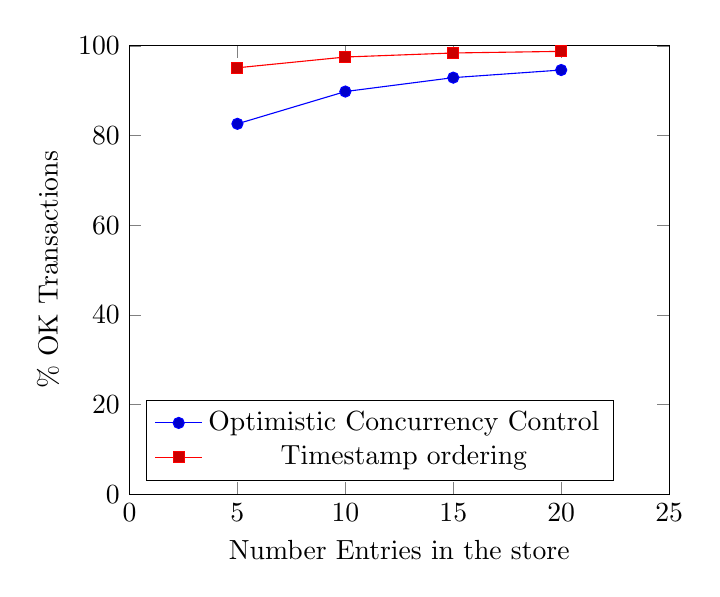
\begin{tikzpicture}
    \begin{axis}
      [
      xlabel={Number Entries in the store},
      ylabel={\% OK Transactions},
      xmin=0, xmax=25,
      ymin=0, ymax=100,
      scaled x ticks = true,
      scaled y ticks = true,
      legend pos= south west,
      ]
      \addplot coordinates {
        (5,82.6)
        (10,89.8)
        (15,92.9)
        (20,94.6)
     };
     \addplot coordinates {
     (5,95.1)
     (10,97.5)
     (15,98.4)
     (20,98.76)
    };
    \addlegendentry{Optimistic Concurrency Control}
    \addlegendentry{Timestamp ordering}
    \end{axis}
  \end{tikzpicture}
  \captionof{figure}{Relation between number of entries and Ok Transactions}
  \label{fig:timey_graph_entries}
\end{minipage}

\textbf{Answer:} Using both algorithms the success rate is really high, even
increasing the number of entries in the store. The success rate is quite better
when the number of entries get bigger, but is not a really significant change.
The reason this happens is that the bigger the number the entries, less entry
conflicts have the clients for each entry.\\\\

\textit{Timestamp ordering}, as in the previous section, has better success rate than \textit{Optimistic concurrency control}.

\item \textbf{Question:} Different number of read operations per transaction\\\\
  
\begin{minipage}[H]{\linewidth}
  \centering
  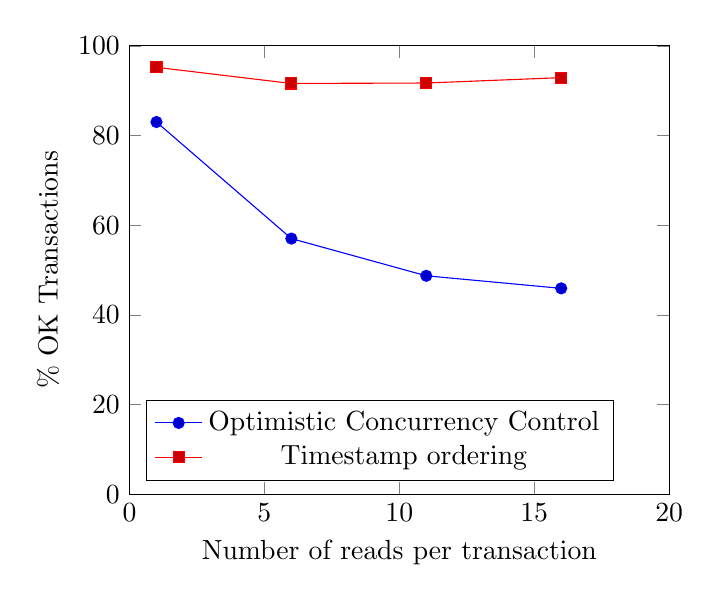
\begin{tikzpicture}
    \begin{axis}
      [
      xlabel={Number of reads per transaction},
      ylabel={\% OK Transactions},
      xmin=0, xmax=20,
      ymin=0, ymax=100,
      scaled x ticks = true,
      scaled y ticks = true,
      legend pos= south west,
      ]
      \addplot coordinates {
    (1,83)
    (6,57)
    (11,48.7)
    (16,45.9)
     };
     \addplot coordinates {

     (1,95.2)
     (6,91.6)
     (11,91.7)
     (16,92.9)
    };
    \addlegendentry{Optimistic Concurrency Control}
    \addlegendentry{Timestamp ordering}
    \end{axis}
  \end{tikzpicture}
  \captionof{figure}{Relation between number of reads per transaction and Ok Transactions}
  \label{fig:timey_graph_entries}
\end{minipage}

\textbf{Answer:} In this case, still there is a reaffirmation that the \textit{Timestamp ordering} is a better solution for this testbed. In this experiment, as we increase the number of reads per transaction, the success rate gets smaller in the \textit{Optimistic concurrency control} algorithm while the timestamp algorithm maintains it's success rate in approximatelly 92\%.


\item \textbf{Question:} Different number of write operations per transaction\\\\

\begin{minipage}[H]{\linewidth}
  \centering
  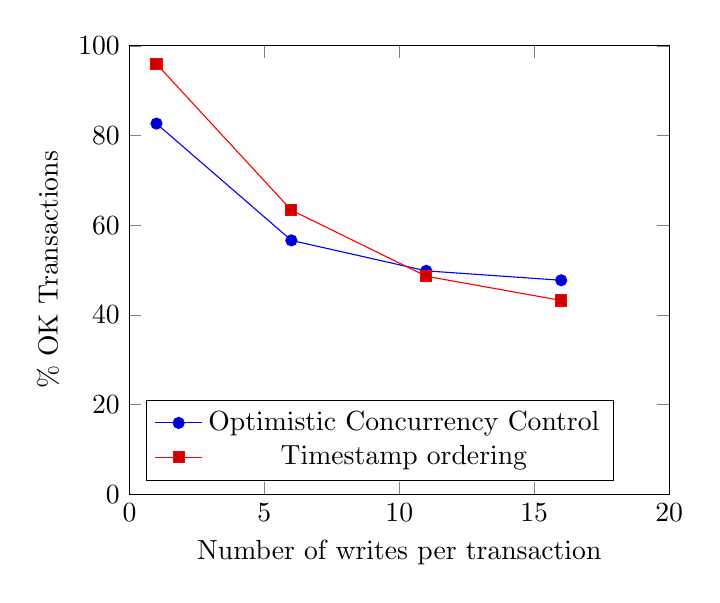
\begin{tikzpicture}
    \begin{axis}
      [
      xlabel={Number of writes per transaction},
      ylabel={\% OK Transactions},
      xmin=0, xmax=20,
      ymin=0, ymax=100,
      scaled x ticks = true,
      scaled y ticks = true,
      legend pos= south west,
      ]
      \addplot coordinates {

      (1,82.65)
      (6,56.6)
      (11,49.8)
      (16,47.7)
     };
     \addplot coordinates {

       (1,95.95)
       (6,63.34)
       (11,48.6)
       (16,43.2)
    };
    \addlegendentry{Optimistic Concurrency Control}
    \addlegendentry{Timestamp ordering}
    \end{axis}
  \end{tikzpicture}
  \captionof{figure}{Relation between number of writes per transaction and Ok Transactions}
  \label{fig:timey_graph_writes}
\end{minipage}

\textbf{Answer:} This is the most conflicting experiment, it proves that both concurrency control protocols are better depending on the different number of writes per transaction. In all previous scenarios, the \textit{Timestamp ordering} protocol was getting better results. In this one, it happens until the number of writes per transaction is approximatelly 11. From there, the \textit{Optimistic} protocol get a slightly better results.


\item \textbf{Question:} Different ratio of reads and writes operations per transaction\\\\


\begin{minipage}[H]{\linewidth}
  \centering
  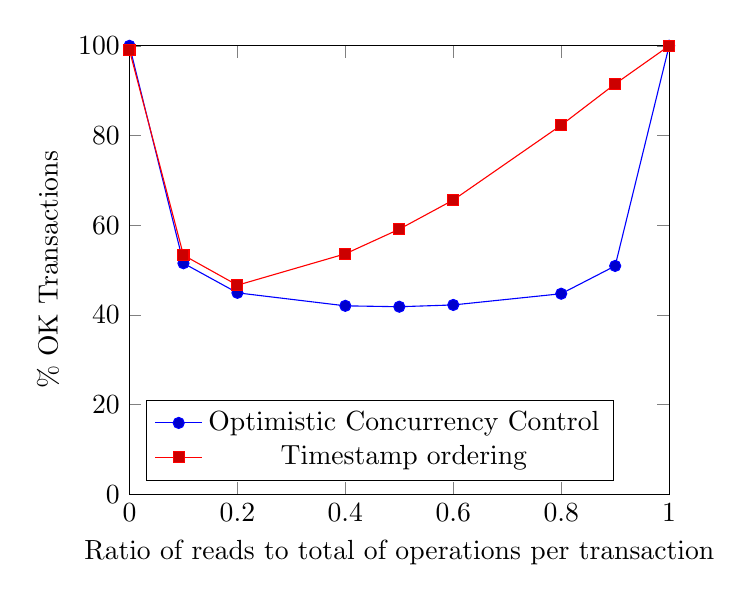
\begin{tikzpicture}
    \begin{axis}
      [
      xlabel={Ratio of reads to total of operations per transaction},
      ylabel={\% OK Transactions},
      xmin=0, xmax=1,
      ymin=0, ymax=100,
      scaled x ticks = true,
      scaled y ticks = true,
      legend pos= south west,
      ]
      \addplot coordinates {
      (0,100)
      (0.1,51.5)
      (0.2,44.9)
      (0.4,42)
      (0.5,41.8)
      (0.6,42.2)
      (0.8,44.7)
      (0.9,50.9)
      (1,100)

     };
     \addplot coordinates {
     (0,99)
     (0.1,53.3)
     (0.2,46.6)
     (0.4,53.6)
     (0.5,59.1)
     (0.6,65.6)
     (0.8,82.3)
     (0.9,91.5)
     (1,100)

    };
    \addlegendentry{Optimistic Concurrency Control}
    \addlegendentry{Timestamp ordering}
    \end{axis}
  \end{tikzpicture}
  \captionof{figure}{Relation between ratio of read and write per transaction and Ok Transactions}
  \label{fig:timey_graph_ratio}
\end{minipage}

\textbf{Answer:} In this scenario, the \textit{timestamp ordering} protocol follows a different function than the \textit{Optimistic concurrency} one. Given a fixed number of operations and changing the ratio of reads towards writes for each transaction, the \textit{Optimistic concurrency} performs a simetric function. The \textit{timestamp ordering}, in the other hand, seems to be more like an exponential increase starting from the experiment where there is at least one read.

\end{enumerate}

\subsection{Conclusion}

After performing all the experiments using both algorithms, we have clearly seen that the \textit{timestamp ordering} protocol is a little bit better than the \textit{optimistic concurrency control} protocol. The main difference we have seen between them is that the \textit{timestamp ordering} validates the transaction at the same moment it performs the operations while the \textit{optimistic concurrency control} has three phases in each transaction and only validates at the end. This means there is more time per transaction without been validated, so there is more probability of conflicts.

\section{Personal opinion}
For this project, we had some advantage because we were already familiarized
with the environment. In our opinion, the algorithm was easy to implement than
PAXY and we have had more time to test the behaviour subject to different
parameters. We have enjoyed plying with the number of clients, entries, messages
sent, etc. while comparing the effect on the performance between a base case and
versus another algorithm (Timey). Maybe, this seminar would fit better as the
first one since the algorithm itself is easier to understand and there is less
code to develop in comparison to PAXY. Nevertheless, we were able to simulate a
real Optimistic concurrency control method and see it running and we appreciate
that. Lately, we have seen other methods that would be also interesting
to use as comparison (for instance strict-two phase locking) or even testing
alongside different consistency models.

\section{Appendix - Experiment Tables}

\subsection{Different number of clients table}

 \begin{table}[H]
    \begin{tabular}{ |c|c|c|c| }
      \hline
      \multicolumn{4}{|c|}{Concurrent Clients - Duration 3s} \\
      \hline
      Experiment & Total Transactions & OK Transactions & \% Transactions\\
      \hline
      \multirow{4}{3cm}{3 CLIENTS \\ 5 ENTRIES \\ 1 RDxTR \\ 1 WRxTR}
      & 96608 & 79630 & 82.4258860549851 \%\\
      & 96489 & 79571 & 82.46639513312398 \%\\
      & 96447 & 79510 & 82.43905979449853 \%\\
      & & &\\
      \hline
      \multirow{8}{3cm}{8 CLIENTS \\ 5 ENTRIES \\ 1 RDxTR \\ 1 WRxTR}
      & 49812 & 28991 &  58.20083514012688 \%\\
      & 49882 & 28951 &  58.0389719738583 \%\\
      & 49885 & 29002 &  58.1377167485216 \%\\
      & 49827 & 28862 &  57.92441848796837 \%\\
      & 49722 & 28978 &  58.28003700575198 \%\\
      & 49810 & 28866 &  57.95221843003413 \%\\
      & 49813 & 28816 &  57.848352839620176 \%\\
      & 49757 & 28796 &  57.87326406334787 \%\\ 
      \hline
      \multirow{13}{3cm}{13 CLIENTS \\ 5 ENTRIES \\ 1 RDxTR \\ 1 WRxTR}
      & 31501 & 14260 &  45.26840417764515 \%\\
      & 31480 & 14244 &  45.247776365946635 \%\\
      & 31545 & 14269 &  45.233792994135364 \%\\
      & 31553 & 14332 &  45.421988400469054 \%\\
      & 31543 & 14317 &  45.38883428969977 \%\\
      & 31542 & 14349 &  45.49172531862279 \%\\
      & 31521 & 14275 &  45.2872688049237 \%\\
      & 31533 & 14266 &  45.24149303903847 \%\\
      & 31551 & 14147 &  44.83851541947957 \%\\
      & 31558 & 14239 &  45.12009633056594 \%\\
      & 31542 & 14364 &  45.539280958721704 \%\\
      & 31544 & 14317 &  45.38739538422521 \%\\
      & 31587 & 14258 &  45.138822933485294 \%\\
      \hline
      \multirow{18}{3cm}{18 CLIENTS \\ 5 ENTRIES \\ 1 RDxTR \\ 1 WRxTR}
      & 22777 & 8668 &  38.055933617245465 \%\\
      & 22790 & 8652 &  37.96401930671347 \%\\
      & 22799 & 8804 &  38.615728760033335 \%\\
      & 22820 & 8714 &  38.185801928133216 \%\\
      & 22781 & 8611 &  37.79904306220096 \%\\
      & 22812 & 8624 &  37.80466421181834 \%\\
      & 22793 & 8708 &  38.20471197297416 \%\\
      & 22775 & 8740 &  38.375411635565314 \%\\
      & 22779 & 8664 &  38.03503226656131 \%\\
      & 22758 & 8678 &  38.13164601458828 \%\\
      & 22795 & 8609 &  37.76705417854793 \%\\
      & 22801 & 8679 &  38.06411999473707 \%\\
      & 22779 & 8550 &  37.5345713156855 \%\\
      & 22817 & 8689 &  38.08125520445282 \%\\
      & 22797 & 8739 &  38.33399131464667 \%\\
      & 22803 & 8743 &  38.34144630092532 \%\\
      & 22793 & 8743 &  38.35826788926425 \%\\
      & 22790 & 8586 &  37.674418604651166 \%\\
      \hline
    \end{tabular}
    \captionof{figure}{Different number of Concurrent clients - Duration 3s}
    \label{table:diff_clients}
  \end{table}
 

\subsection{Different number of entries table}

\begin{table}[H]
\begin{tabular}{ |c|c|c|c| }
  \hline
  \multicolumn{4}{|c|}{Concurrent Clients - Duration 3s} \\
  \hline
  Experiment & Total Transactions & OK Transactions & \% Transactions\\
  \hline
  \multirow{4}{3cm}{3 CLIENTS \\ 5 ENTRIES \\ 1 RDxTR \\ 1 WRxTR}
  & 140798 & 116289 &  82.59279251125726 \%\\
  & 141163 & 116802 &  82.7426450273797 \%\\
  & 141246 & 116576 &  82.5340186624754 \%\\
  & & &\\
  \hline
  \multirow{4}{3cm}{3 CLIENTS \\ 10 ENTRIES \\ 1 RDxTR \\ 1 WRxTR}
  & 138150 & 124355 &  90.01447701773435 \%\\
  & 138452 & 124431 &  89.87302458613816 \%\\
  & 138136 & 124077 &  89.82234898940175 \%\\
  & & &\\
  \hline

  \multirow{4}{3cm}{3 CLIENTS \\ 15 ENTRIES \\ 1 RDxTR \\ 1 WRxTR}
  & 132575 & 123248 &  92.96473694135395 \%\\
  & 132549 & 123307 &  93.02748417566335 \%\\
  & 132296 & 122918 &  92.91135030537582 \%\\
  & & &\\
  \hline

  \multirow{4}{3cm}{3 CLIENTS \\ 20 ENTRIES \\ 1 RDxTR \\ 1 WRxTR}
  & 127943 & 121099 &  94.65074290895164 \%\\
  & 127604 & 120619 &  94.52603366665622 \%\\
  & 127395 & 120505 &  94.59162447505788 \%\\
  & & &\\
  \hline

\end{tabular}
\captionof{figure}{Results of several executions changing the number of entries}
\label{table:acceptorsDelay}
\end{table}

\subsection{Different number of reads per transaction table}

  \begin{table}[H]
  \begin{tabular}{ |c|c|c|c| }
    \hline
    \multicolumn{4}{|c|}{Read Operations - Duration 3s} \\
    \hline
    Experiment & Total Transactions & OK Transactions & \% Transactions\\
    \hline
    \multirow{4}{3cm}{3 CLIENTS \\ 5 ENTRIES \\ 1 RDxTR \\ 1 WRxTR}
     & 142142 & 117720 &  82.81858986084339 \%\\
     & 141947 & 117419 &  82.72031110203103 \%\\
     & 141938 & 117234 &  82.59521763023292 \%\\
     & & &\\
    \hline
    \multirow{4}{3cm}{3 CLIENTS \\ 5 ENTRIES \\ 6 RDxTR \\ 1 WRxTR}
    & 52637 & 29805 &  56.62366776222049 \%\\
    & 52699 & 30052 &  57.02575001423177 \%\\
    & 52441 & 29173 &  55.63013672508152 \%\\
    & & &\\
    \hline
    \multirow{4}{3cm}{3 CLIENTS \\ 5 ENTRIES \\ 11 RDxTR \\ 1 WRxTR}
    & 31854 & 15446 &  48.48998555911346 \%\\
    & 31813 & 15160 &  47.653474994499106 \%\\
    & 31861 & 15543 &  48.783779542387244 \%\\
    & & &\\
    \hline
    \multirow{4}{3cm}{3 CLIENTS \\ 5 ENTRIES \\ 16 RDxTR \\ 1 WRxTR}
     & 22665 & 10067 &  44.41650121332451 \%\\
     & 22658 & 10198 &  45.0083855591844 \%\\
     & 22680 & 10417 &  45.930335097001766 \%\\
    & & &\\
    \hline
 
 \end{tabular}
  \captionof{figure}{Different number of Transactions Reads - Duration 3s}
  \label{table:diff_rdtx}
\end{table}



\subsection{Different number of writes per transaction table}

\begin{table}[H]
\begin{tabular}{ |c|c|c|c| }
  \hline
  \multicolumn{4}{|c|}{Concurrent Clients - Duration 3s} \\
  \hline
  Experiment & Total Transactions & OK Transactions & \% Transactions\\
  \hline
  \multirow{4}{3cm}{3 CLIENTS \\ 5 ENTRIES \\ 1 RDxTR \\ 1 WRxTR}
  & 141785 & 117116 &  82.60112141622879 \%\\
  & 141855 & 117186 &  82.60970709527334 \%\\
  & 142148 & 117599 &  82.72997157891774 \%\\
  & & &\\
  \hline
  \multirow{4}{3cm}{3 CLIENTS \\ 5 ENTRIES \\ 1 RDxTR \\ 6 WRxTR}
  & 109430 & 61814 &  56.48725212464589 \%\\
  & 109888 & 62411 &  56.79510046592895 \%\\
  & 109707 & 61964 &  56.48135488163928 \%\\
  & & &\\
  \hline

  \multirow{4}{3cm}{3 CLIENTS \\ 5 ENTRIES \\ 1 RDxTR \\ 11 WRxTR}
  & 95094 & 47591 &  50.04627000651986 \%\\
  & 95056 & 47466 &  49.93477529035516 \%\\
  & 95183 & 47182 &  49.56977611548281 \%\\
  & & &\\
  \hline

  \multirow{4}{3cm}{3 CLIENTS \\ 5 ENTRIES \\ 1 RDxTR \\ 16 WRxTR}
  & 80710 & 38710 &  47.961838681699916 \%\\
  & 80633 & 38254 &  47.44211427083204 \%\\
  & 80680 & 38514 &  47.73673772930094 \%\\
  & & &\\
  \hline
\end{tabular}
\captionof{figure}{Results of several executions changing the number of write operations per transaction}
\label{table:acceptorsDelay}
\end{table}

\newpage
\subsection{Different ratio of reads and writes per transaction table}

  \begin{table}[H]
  \begin{tabular}{ |c|c|c|c| }
    \hline
    \multicolumn{4}{|c|}{Ratio Read/Write Operations - Duration 3s} \\
    \hline
    Experiment & Total Transactions & OK Transactions & \% Transactions\\
    \hline
    \multirow{4}{3cm}{3 CLIENTS \\ 5 ENTRIES \\ 1 RDxTR \\ 1 WRxTR}
    & 143527 & 118318 &  82.4360573271928 \%\\
    & 143478 & 118841 &  82.82872635526005 \%\\
    & 143232 & 118496 &  82.7301161751564 \%\\
    & & &\\
    \hline
    \multirow{4}{3cm}{3 CLIENTS \\ 5 ENTRIES \\ 0 RDxTR \\ 10 WRxTR}
    & 139160 & 139160 &  100.0 \%\\
    & 139216 & 139216 &  100.0 \%\\
    & 138848 & 138848 &  100.0 \%\\
    & & &\\
    \hline
    \multirow{4}{3cm}{3 CLIENTS \\ 5 ENTRIES \\ 2 RDxTR \\ 8 WRxTR}
     & 85776 & 38770 &  45.199123297892186 \%\\
     & 85789 & 38354 &  44.70736341489002 \%\\
     & 85615 & 38244 &  44.66974245167319 \%\\
    & & &\\
    \hline
    \multirow{4}{3cm}{3 CLIENTS \\ 5 ENTRIES \\ 4 RDxTR \\ 6 WRxTR}
    & 65387 & 27501 & 42.058819031305916 \%\\
    & 65306 & 27684 & 42.3912044835084 \%\\
    & 65390 & 27448 & 41.975837283988376 \%\\
    & & &\\
    \hline
    \multirow{4}{3cm}{3 CLIENTS \\ 5 ENTRIES \\ 5 RDxTR \\ 5 WRxTR}
    & 58562 & 24337 &  41.55766538028073 \%\\
    & 58558 & 24596 &  42.002800642098435 \%\\
    & 58670 & 25021 &  42.64700869268791 \%\\
    & & &\\
    \hline
    \multirow{4}{3cm}{3 CLIENTS \\ 5 ENTRIES \\ 6 RDxTR \\ 4 WRxTR}
    & 54417 & 22837 &  41.966664829005644 \%\\
    & 54407 & 22909 &  42.10671420956862 \%\\
    & 54403 & 23174 &  42.596915611271434 \%\\
    & & &\\
    \hline
    \multirow{4}{3cm}{3 CLIENTS \\ 5 ENTRIES \\ 8 RDxTR \\ 2 WRxTR}
    & 44222 & 19690 &  44.525349373614944 \%\\
    & 44194 & 19618 &  44.39064126351993 \%\\
    & 44175 & 19589 &  44.344086021505376 \%\\
    & & &\\
    \hline
    \multirow{4}{3cm}{3 CLIENTS \\ 5 ENTRIES \\ 10 RDxTR \\ 0 WRxTR}
     & 31749 & 31749 &  100.0 \%\\
     & 31716 & 31716 &  100.0 \%\\
     & 31690 & 31690 &  100.0 \%\\
    & & &\\
    \hline
 \end{tabular}
  \captionof{figure}{Different ratio Read/Writes Operations - Duration 3s}
  \label{table:diff_ratio_read_write}
\end{table}


\subsection{Different percentage of accessed entries with respect to the total number of entries}
\begin{table}[H]
\begin{tabular}{ |c|c|c|c| }
  \hline
  \multicolumn{4}{|c|}{Concurrent Clients - Duration 3s} \\
  \hline
  Experiment & Total Transactions & OK Transactions & \% Transactions\\
  \hline

  \multirow{5}{4cm}{3 CLIENTS \\ 5 ENTRIES \\ 1 RDxTR \\ 1 WRxTR \\ 5 ENTRIES/CLIENT}
  & 142536 & 117794 &  82.64157826794634 \%\\
  & 142789 & 117943 &  82.59949996148163 \%\\
  & 142512 & 117855 &  82.6982990906029 \%\\
  & & &\\
  & & &\\
  \hline

  \multirow{5}{4cm}{3 CLIENTS \\ 5 ENTRIES \\ 1 RDxTR \\ 6 WRxTR \\ 4 ENTRIES/CLIENT}
  & 114353 & 66215 &  57.90403399998251 \%\\
  & 113979 & 74988 &  65.79106677545863 \%\\
  & 113896 & 65381 &  57.40412305963335 \%\\
  & & &\\
  & & &\\
  \hline

  \multirow{5}{4cm}{3 CLIENTS \\ 5 ENTRIES \\ 1 RDxTR \\ 11 WRxTR \\ 3 ENTRIES/CLIENT}
  & 101740 & 68126 &  66.96088067623354 \%\\
  & 102144 & 57387 &  56.18244830827068 \%\\
  & 102121 & 57234 &  56.04527961927517 \%\\
  & & &\\
  & & &\\
  \hline

  \multirow{5}{4cm}{3 CLIENTS \\ 5 ENTRIES \\ 1 RDxTR \\ 16 WRxTR \\ 2 ENTRIES/CLIENT}
  & 90919 & 78709 &  86.57046381944367 \%\\
  & 91111 & 54920 &  60.278122290393036 \%\\
  & 90759 & 78383 &  86.36388677706894 \%\\
  & & &\\
  & & &\\
  \hline

  \multirow{5}{4cm}{3 CLIENTS \\ 5 ENTRIES \\ 1 RDxTR \\ 16 WRxTR \\ 10 ENTRIES/CLIENT}
  & 70885 & 39096 &  55.15412287507935 \%\\
  & 70628 & 42511 &  60.19000962790961 \%\\
  & 70478 & 45097 &  63.98734356820568 \%\\
  & & &\\
  & & &\\
  \hline

  \multirow{5}{4cm}{3 CLIENTS \\ 5 ENTRIES \\ 1 RDxTR \\ 16 WRxTR \\ 7 ENTRIES/CLIENT}
  & 74117 & 50234 &  67.77662344671263 \%\\
  & 73891 & 50030 &  67.70783992637804 \%\\
  & 74195 & 45022 &  60.68063885706584 \%\\
  & & &\\
  & & &\\
  \hline

  \multirow{5}{4cm}{3 CLIENTS \\ 5 ENTRIES \\ 1 RDxTR \\ 16 WRxTR \\ 3 ENTRIES/CLIENT}
  & 82839 & 70800 &  85.46699018578207 \%\\
  & 83198 & 71080 &  85.43474602754874 \%\\
  & 82806 & 82806 &  100.0 \%\\
  & & &\\
  & & &\\
  \hline

  \multirow{5}{4cm}{3 CLIENTS \\ 5 ENTRIES \\ 1 RDxTR \\ 16 WRxTR \\ 2 ENTRIES/CLIENT}
  & 89473 & 89473 &  100.0 \%\\
  & 89588 & 73283 &  81.80001785953476 \%\\
  & 89691 & 72726 &  81.08505870154197 \%\\
  & & &\\
  & & &\\
  \hline

\end{tabular}

\captionof{figure}{Results of several executions changing the percentage of accessed entries with respect to the total number of entries}
\label{table:acceptorsDelay}
\end{table}

\subsection{[Timestamp ordering] Different number of clients table}

\begin{table}[H]
\begin{tabular}{ |c|c|c|c| }
  \hline
  \multicolumn{4}{|c|}{Concurrent Clients - Duration 3s} \\
  \hline
  Experiment & Total Transactions & OK Transactions & \% Transactions\\
  \hline
  \multirow{4}{3cm}{3 CLIENTS \\ 5 ENTRIES \\ 1 RDxTR \\ 1 WRxTR}
  & 95846 & 91049 &  94.99509630031508 \%\\
  & 95921 & 91253 &  95.13349527215104 \%\\
  & 95735 & 91007 &  95.06136731602862 \%\\
  & & &\\
  \hline
  \multirow{8}{3cm}{8 CLIENTS \\ 5 ENTRIES \\ 1 RDxTR \\ 1 WRxTR}
  & 40681 & 34438 &  84.65376957301935 \%\\
  & 40468 & 34183 &  84.46921024018978 \%\\
  & 40652 & 34386 &  84.5862442192266 \%\\
  & 40685 & 34367 &  84.47093523411577 \%\\
  & 40562 & 34355 &  84.69750012326809 \%\\
  & 40761 & 34513 &  84.6716223841417 \%\\
  & 40566 & 34346 &  84.66696248089534 \%\\
  & 40694 & 34421 &  84.58495109844203 \%\\
  \hline

  \multirow{13}{3cm}{13 CLIENTS \\ 5 ENTRIES \\ 1 RDxTR \\ 1 WRxTR}
  & 26690 & 20729 &  77.66579243162234 \%\\
  & 26656 & 20670 &  77.54351740696279 \%\\
  & 26706 & 20640 &  77.2860031453606 \%\\
  & 26709 & 20742 &  77.65921599460856 \%\\
  & 26708 & 20904 &  78.2686835405122 \%\\
  & 26706 & 20867 &  78.13599940088369 \%\\
  & 26700 & 20695 &  77.50936329588015 \%\\
  & 26793 & 20880 &  77.93080282163251 \%\\
  & 26782 & 20736 &  77.42513628556493 \%\\
  & 26794 & 20845 &  77.79726804508472 \%\\
  & 26742 & 20691 &  77.37267220103209 \%\\
  & 26683 & 20554 &  77.03031892965559 \%\\
  & 26779 & 20879 &  77.96781059785653 \%\\
  \hline

  \multirow{18}{3cm}{18 CLIENTS \\ 5 ENTRIES \\ 1 RDxTR \\ 1 WRxTR}
  & 19381 & 14309 &  73.83003972963212 \%\\
  & 19363 & 14313 &  73.91933068222899 \%\\
  & 19449 & 14268 &  73.36109825697979 \%\\
  & 19447 & 14279 &  73.42520697279787 \%\\
  & 19361 & 14249 &  73.59640514436238 \%\\
  & 19431 & 14377 &  73.99001595388812 \%\\
  & 19310 & 14275 &  73.92542723977213 \%\\
  & 19470 & 14494 &  74.4427324088341 \%\\
  & 19367 & 14156 &  73.09340630970208 \%\\
  & 19388 & 14219 &  73.33917887353002 \%\\
  & 19384 & 14279 &  73.66384647131655 \%\\
  & 19342 & 14254 &  73.69455071864337 \%\\
  & 19420 & 14373 &  74.01132852729145 \%\\
  & 19271 & 14125 &  73.2966633802086 \%\\
  & 19273 & 14143 &  73.3824521351113 \%\\
  & 19461 & 14390 &  73.94275730949077 \%\\
  & 19478 & 14404 &  73.95009754594928 \%\\
  & 19314 & 14169 &  73.36129232680956 \%\\
  \hline
\end{tabular}
\captionof{figure}{Results of several executions changing the number of clients in the Timestamp ordering algorithm}
\label{table:timey_change_clients}
\end{table}
\subsection{[Timestamp ordering] Different number of entries table}

\begin{table}[H]
\begin{tabular}{ |c|c|c|c| }
  \hline
  \multicolumn{4}{|c|}{Concurrent Clients - Duration 3s} \\
  \hline
  Experiment & Total Transactions & OK Transactions & \% Transactions\\
  \hline
  \multirow{4}{3cm}{3 CLIENTS \\ 5 ENTRIES \\ 1 RDxTR \\ 1 WRxTR}
  & 83714 & 79750 &  95.26483025539336 \%\\
  & 83462 & 79407 &  95.14150152165057 \%\\
  & 83683 & 79722 &  95.26666109006608 \%\\
  & & &\\
  \hline
  \multirow{4}{3cm}{3 CLIENTS \\ 10 ENTRIES \\ 1 RDxTR \\ 1 WRxTR}
  & 86061 & 83926 &  97.51920149661287 \%\\
  & 86258 & 84141 &  97.54573488835818 \%\\
  & 86285 & 84142 &  97.51637016862722 \%\\
  & & &\\
  \hline

  \multirow{4}{3cm}{3 CLIENTS \\ 15 ENTRIES \\ 1 RDxTR \\ 1 WRxTR}
  & 85535 & 84107 &  98.3305079791898 \%\\
  & 85691 & 84365 &  98.45257961746275 \%\\
  & 85738 & 84447 &  98.49424992418764 \%\\
  & & &\\

  \hline

  \multirow{4}{3cm}{3 CLIENTS \\ 20 ENTRIES \\ 1 RDxTR \\ 1 WRxTR}
  & 86984 & 85927 &  98.78483399245839 \%\\
  & 86733 & 85650 &  98.75134032029331 \%\\
  & 86756 & 85695 &  98.7770298307898 \%\\
  & & &\\

  \hline
\end{tabular}
\captionof{figure}{Results of several executions changing the number of entries in the Timestamp ordering algorithm}
\label{table:timey_change_entries}
\end{table}


\subsection{[Timestamp ordering] Different number of reads per transaction table}

\begin{table}[H]
\begin{tabular}{ |c|c|c|c| }
  \hline
  \multicolumn{4}{|c|}{Concurrent Clients - Duration 3s} \\
  \hline
  Experiment & Total Transactions & OK Transactions & \% Transactions\\
  \hline
  \multirow{4}{3cm}{3 CLIENTS \\ 5 ENTRIES \\ 1 RDxTR \\ 1 WRxTR}
  & 84802 & 80827 &  95.31261055163793 \%\\
  & 84585 & 80552 &  95.23201513270675 \%\\
  & 84694 & 80737 &  95.32788627293552 \%\\
  & & &\\
  \hline
  \multirow{4}{3cm}{3 CLIENTS \\ 5 ENTRIES \\ 6 RDxTR \\ 1 WRxTR}
  & 32364 & 29636 &  91.57088122605364 \%\\
  & 32377 & 29713 &  91.77193686876487 \%\\
  & 32353 & 29532 &  91.28056130807035 \%\\
  & & &\\
  \hline

  \multirow{4}{3cm}{3 CLIENTS \\ 5 ENTRIES \\ 11 RDxTR \\ 1 WRxTR}
  & 19417 & 17853 &  91.9452026574651 \%\\
  & 19428 & 17825 &  91.7490220300597 \%\\
  & 19403 & 17777 &  91.61985260011339 \%\\
  & & &\\

  \hline

  \multirow{4}{3cm}{3 CLIENTS \\ 5 ENTRIES \\ 16 RDxTR \\ 1 WRxTR}


  & 13542 & 12612 &  93.13247673903412 \%\\
  & 13548 & 12568 &  92.76645999409507 \%\\
  & 13545 & 12571 &  92.80915466961979 \%\\
  & & &\\
  \hline
\end{tabular}
\captionof{figure}{Results of several executions changing the number of reads per transaction in the Timestamp ordering algorithm}
\label{table:timey_change_reads}
\end{table}

\subsection{[Timestamp ordering] Different number of writes per transaction table}

\begin{table}[H]
\begin{tabular}{ |c|c|c|c| }
  \hline
  \multicolumn{4}{|c|}{Concurrent Clients - Duration 3s} \\
  \hline
  Experiment & Total Transactions & OK Transactions & \% Transactions\\
  \hline
  \multirow{4}{3cm}{3 CLIENTS \\ 5 ENTRIES \\ 1 RDxTR \\ 1 WRxTR}

  & 95082 & 90444 &  95.12210513030857 \%\\
  & 95221 & 90584 &  95.13027588452127 \%\\
  & 95247 & 90525 &  95.0423635390091 \%\\
  & & &\\
  \hline
  \multirow{4}{3cm}{3 CLIENTS \\ 5 ENTRIES \\ 1 RDxTR \\ 6 WRxTR}

  & 37820 & 23976 &  63.39502908514014 \%\\
  & 37752 & 23918 &  63.35558381012927 \%\\
  & 37876 & 23942 &  63.21153236878234 \%\\
  & & &\\
  \hline

  \multirow{4}{3cm}{3 CLIENTS \\ 5 ENTRIES \\ 1 RDxTR \\ 11 WRxTR}

  & 26477 & 12763 &  48.204101673150284 \%\\
  & 26405 & 12943 &  49.017231584927096 \%\\
  & 26421 & 12898 &  48.81722871957912 \%\\
  & & &\\
  \hline

  \multirow{4}{3cm}{3 CLIENTS \\ 5 ENTRIES \\ 4 RDxTR \\ 16 WRxTR}
  & 20541 & 8945 &  43.54705223698944 \%\\
  & 20573 & 8844 &  42.98838283186701 \%\\
  & 20514 & 8830 &  43.04377498293848 \%\\
  & & &\\
  \hline
\end{tabular}
\captionof{figure}{Results of several executions changing the number of writes per transaction in the Timestamp ordering algorithm}
\label{table:timey_writes}
\end{table}

\subsection{[Timestamp ordering] Different ratio of reads and writes per transaction table}

\begin{table}[H]
\begin{tabular}{ |c|c|c|c| }
  \hline
  \multicolumn{4}{|c|}{Concurrent Clients - Duration 3s} \\
  \hline
  Experiment & Total Transactions & OK Transactions & \% Transactions\\
  \hline
  \multirow{4}{3cm}{3 CLIENTS \\ 5 ENTRIES \\ 1 RDxTR \\ 1 WRxTR}

  & 96620 & 91978 &  95.19561167460154 \%\\
  & 96765 & 92206 &  95.28858574897949 \%\\
  & 96807 & 92279 &  95.32265228754119 \%\\
  & & &\\
  \hline
  \multirow{4}{3cm}{3 CLIENTS \\ 5 ENTRIES \\ 0 RDxTR \\ 10 WRxTR}
  & 25409 & 25154 &  98.99641859183754 \%\\
  & 25392 & 25151 &  99.05088216761185 \%\\
  & 25403 & 25150 &  99.00405463921584 \%\\
  & & &\\
  \hline

  \multirow{4}{3cm}{3 CLIENTS \\ 5 ENTRIES \\ 2 RDxTR \\ 8 WRxTR}

  & 28972 & 13556 &  46.79000414193014 \%\\
  & 29005 & 13599 &  46.885019824168246 \%\\
  & 28960 & 13397 &  46.2603591160221 \%\\
  & & &\\
  \hline

  \multirow{4}{3cm}{3 CLIENTS \\ 5 ENTRIES \\ 4 RDxTR \\ 6 WRxTR}
  & 27129 & 14496 &  53.43359504589185 \%\\
  & 27150 & 14524 &  53.49539594843462 \%\\
  & 27177 & 14685 &  54.03466166243515 \%\\
  & & &\\
  \hline
  \multirow{4}{3cm}{3 CLIENTS \\ 5 ENTRIES \\ 5 RDxTR \\ 5 WRxTR}
  & 26892 & 16020 &  59.57161981258367 \%\\
  & 26925 & 15989 &  59.38347260909935 \%\\
  & 26906 & 15872 &  58.99055972645507 \%\\
  & & &\\
  \hline

  \multirow{4}{3cm}{3 CLIENTS \\ 5 ENTRIES \\ 6 RDxTR \\ 4 WRxTR}


  & 26953 & 17735 &  65.79972544800208 \%\\
  & 26918 & 17734 &  65.88156623820493 \%\\
  & 26962 & 17795 &  66.00029671389363 \%\\
  & & &\\
  \hline
  \multirow{4}{3cm}{3 CLIENTS \\ 5 ENTRIES \\ 8 RDxTR \\ 2 WRxTR}

  & 26784 & 22065 &  82.38127240143369 \%\\
  & 26737 & 22085 &  82.60089015222351 \%\\
  & 26715 & 21967 &  82.22721317611828 \%\\
  & & &\\
  \hline
  \multirow{4}{3cm}{3 CLIENTS \\ 5 ENTRIES \\ 10 RDxTR \\ 0 WRxTR}

  & 29451 & 29451 &  100.0 \%\\
  & 29483 & 29483 &  100.0 \%\\
  & 29425 & 29425 &  100.0 \%\\
  & & &\\
  \hline

\end{tabular}
\captionof{figure}{Results of several executions changing the ratio if reads and writes per transaction in the Timestamp ordering algorithm}
\label{table:timey_change_ratio}
\end{table}




\end{document}
